\chapter{Surface Simulations Results}
\label{chap:ehd_res}

\section{Introduction}
In the previous chapters, we introduced {\ehd} as a new method to model passivated surfaces in germanium detectors and showed that we can achieve a significant runtime improvement using GPUs. In this chapter, we present the first results from the simulations. The chapter begins with an overview of preprocessing the output waveform, then shows how {\ehd} can be used to simulate varying conditions and match the experimental data from the previous scanners. We then show how the model can be used to estimate the collection efficiency of {\onbb} events and finally demonstrate how it can be used to model background source spectral components with two examples.

\section{Post-Processing and Activeness Maps}
In HPGe detectors, digital filtering is used to determine the energy of each event. The use of a filter can reduce the electronic noise, and thus improve the energy resolution. We applied a trapezoidal filter to the pulse to match one of the techniques used to determine the event energy in the experimental data in LEGEND. Figure \ref{ch5_fig_trap_filter} shows the waveform and trap filter output. Then the energy is picked from the indicated time on the flat top, taken a fixed time after the start time of the pulse's rise. We call the output of the filter the activeness value. Activeness represents the fraction of the initially deposited energy that is collected. Since {\ehd} waveforms are normalized, the activeness values range between 0 and 1, with 0 representing no collection and 1 representing full collection. 

\begin{figure}%[!htb]
\centering
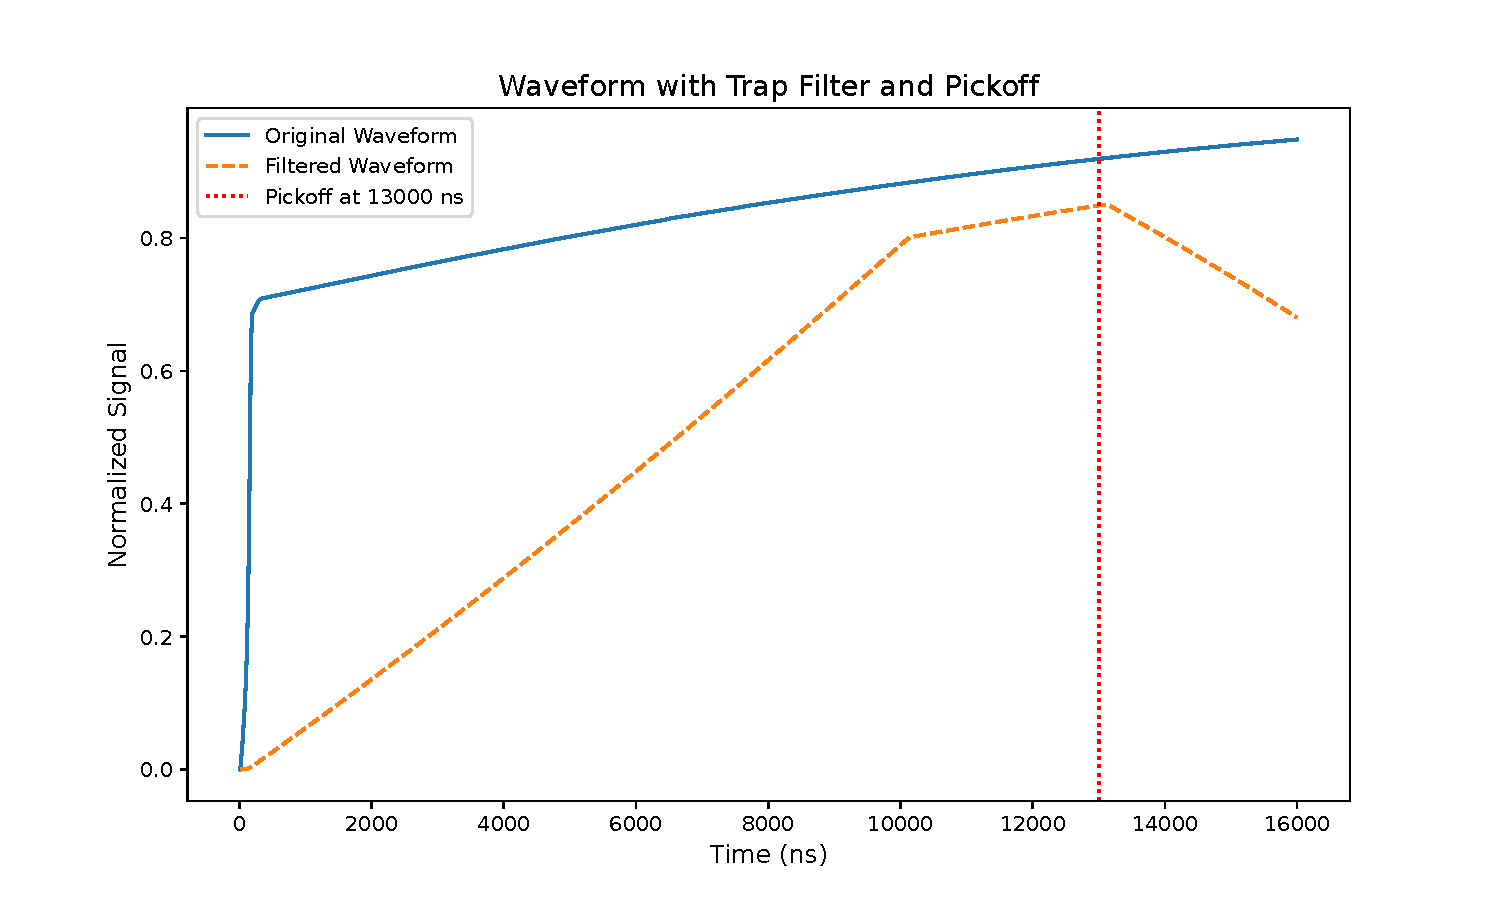
\includegraphics[trim={0cm 0cm 0cm 0cm},clip,width=0.9\linewidth]{ch5/figs/trap_example.pdf}
\caption{A simulated waveform and the resulting trapezoidal filtered waveform for a highly energy degraded surface waveform from {\ehd} simulations. The filter had a rise time of $10 \mu s$, flat time of $3 \mu s$, and the energy estimate is based on the value of the filtered waveform $13 \mu s$ after the start of the pulse rise.}
\label{ch5_fig_trap_filter}
\end{figure}

Although many results in this chapter focus on maps at a single initial energy, the same detector location can exhibit a different partial charge at different energies. 
Figure \ref{ch5_fig_act_eng} shows this variation of activity with initial energy in {\ponama} for various surface charges. The measured activity increases with radius. One possible explanation is that, for higher energy, larger charge clouds are more susceptible to self-repulsion, which can push the charges away from the surface. This means that a smaller fraction of charges is pulled onto the surface in relation to their total number of carriers. Therefore, to accurately model background processes that span a range of energies, we would have to create activeness maps with different positions and initial energies.

\begin{figure}%[!htb]
\centering
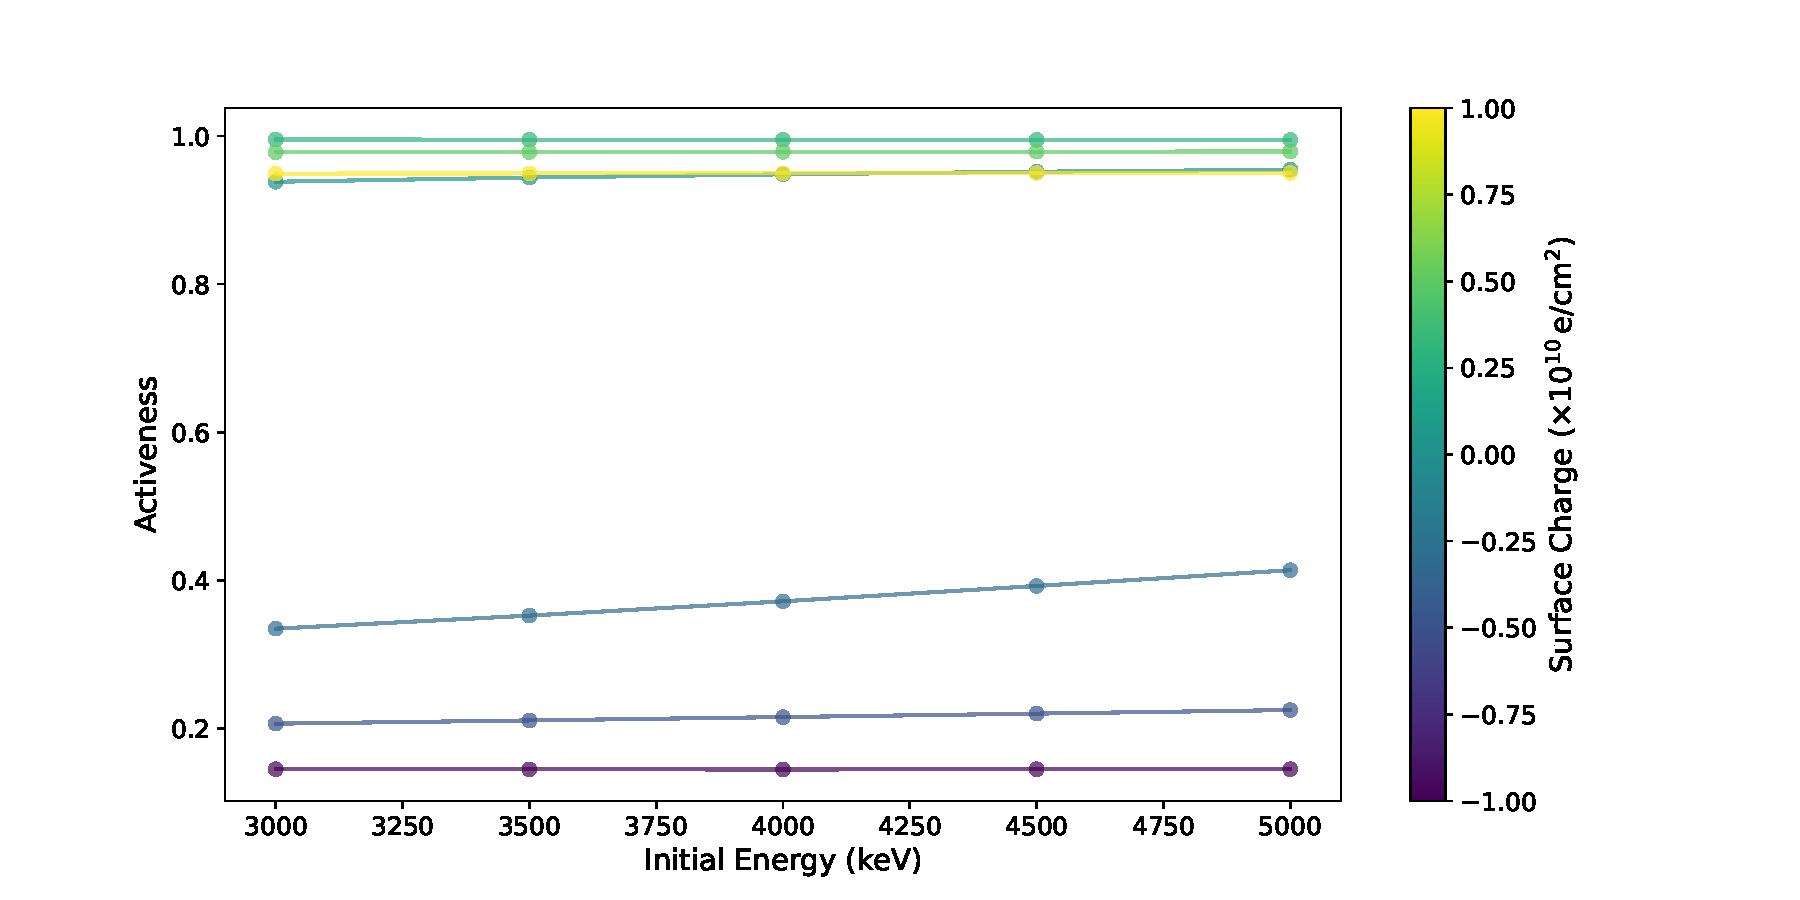
\includegraphics[trim={0cm 0cm 0cm 0cm},clip,width=0.95\linewidth]{ch5/figs/activness_vs_eng.pdf}
\caption{Activeness versus initial energy for event at the same location in {\ponama} detector. The lower activeness loss for higher energy could be due to self repulsion pushing charges away from surface thus leading to smaller fraction of total charges on surface.}
\label{ch5_fig_act_eng}
\end{figure}

To understand the charge collection at different points on the detector, we map the detector using about 100 points, as shown in figure \ref{ch5_fig_activeness_points_neg}. The varying vertical spacing of the points was chosen to accurately capture the behavior in the rapidly varying region nearest to the surface. These points can be used to generate an activeness map for a detector such as in figure \ref{ch5_fig_activeness_map_neg}. This map is produced by interpolating using cubic interpolation. The activeness map gives an understanding of how the charge collection efficiency works in the detectors. Points at the same height but larger radii have a lower activeness, as holes must travel a longer distance, increasing the likelihood of being pulled onto the surface by the negative surface charge. Since each event takes a few minutes to run, it is important to know the optimum number of events needed to sample the map enough for interpolation. We found that approximately 100 points sampled in total in the r and z directions were sufficient.

\begin{figure}%[!htb]
%[trim={left bottom right top},clip]
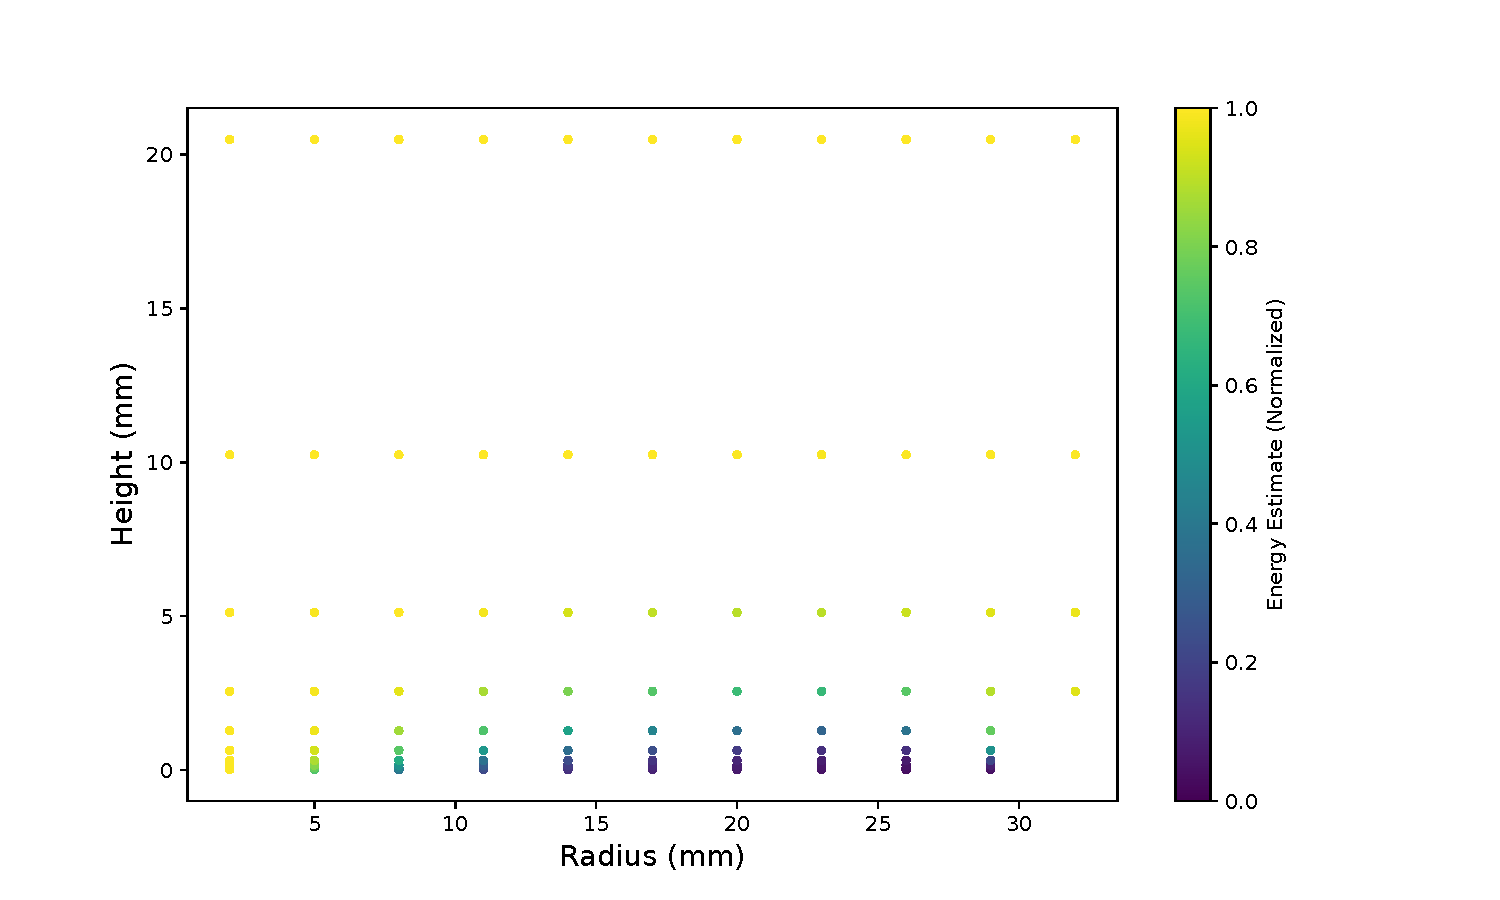
\includegraphics[trim={0cm 0.5cm 3.2cm 1.15cm},clip,width=0.95\linewidth]{ch5/figs/activenss_map_ponama_1_-0.3_5000.pdf}
\caption{Activeness values to map a PPC detector \ehd with an initial energy $5000$ keV and negative surface charge. The radius points were uniformly spaced while the height points were densely sampled close to the surface.}
\label{ch5_fig_activeness_points_neg}
\end{figure}

\begin{figure}%[!htb]
\centering
%[trim={left bottom right top},clip]
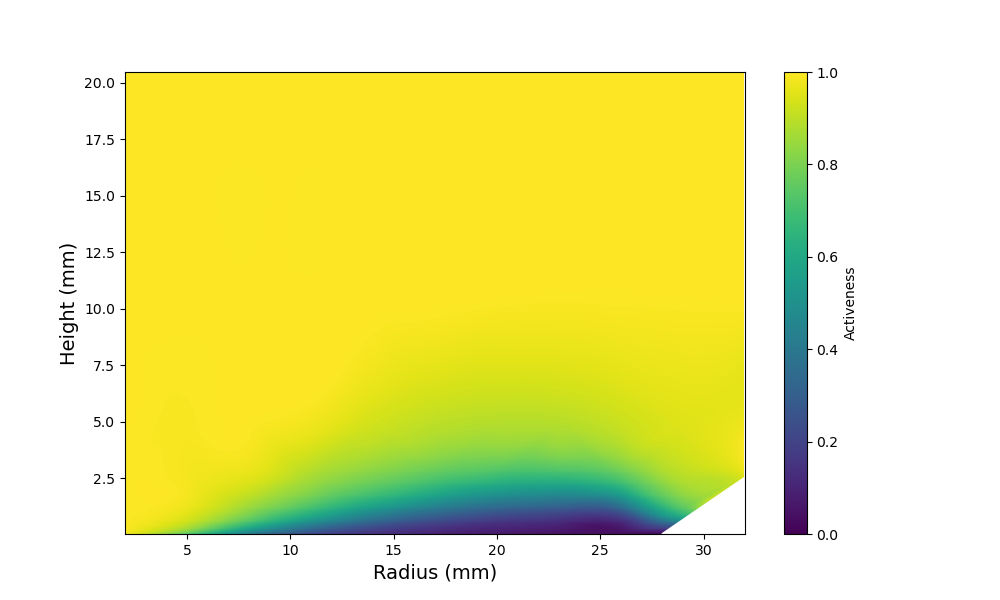
\includegraphics[trim={1.4cm 0.5cm 3.2cm 1.755cm},clip,width=0.95\linewidth]{ch5/figs/activeness_map_cubic_sc=-0.3_ponama_1_5000.png}
% 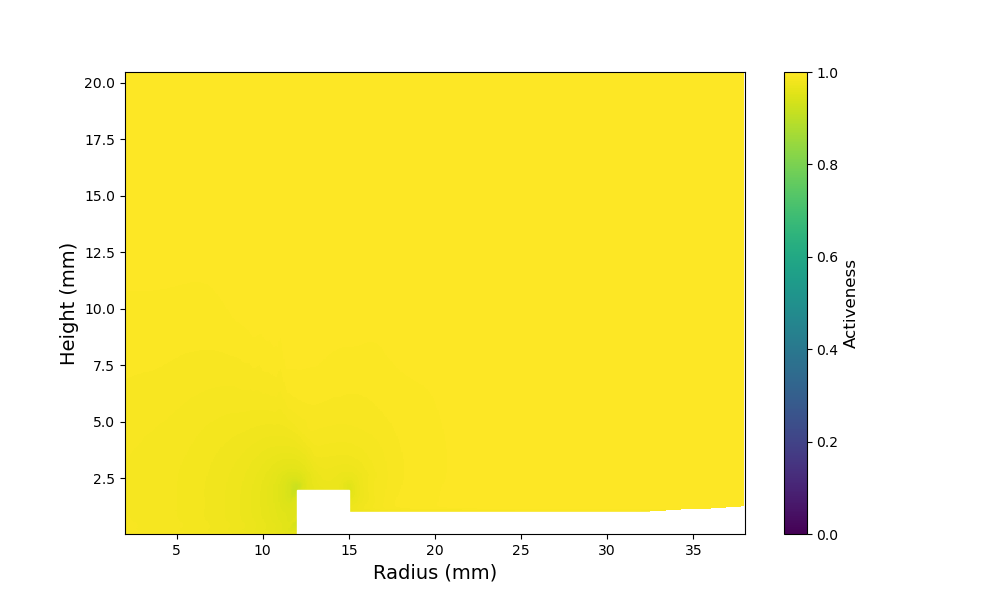
\includegraphics[trim={1.4cm 0.5cm 3.2cm 1.755cm},clip,width=0.49\linewidth]{ch5/figs/activeness_map_cubic_sc=-0.3_V07647A_2039.png}

\caption{Interpolated activeness map for a PPC detector using \ehd with negative surface charge. For a larger radius events there is a higher chance of having the hole component pulled onto the surface, causing higher loss of activeness.}
\label{ch5_fig_activeness_map_neg}
\end{figure}

Figure \ref{ch5_fig_interpolated_activeness_map_0} illustrates the activeness maps without any surface charge. In this case, there is not much reduction in activeness. 

\begin{figure}%[!htb]
\centering
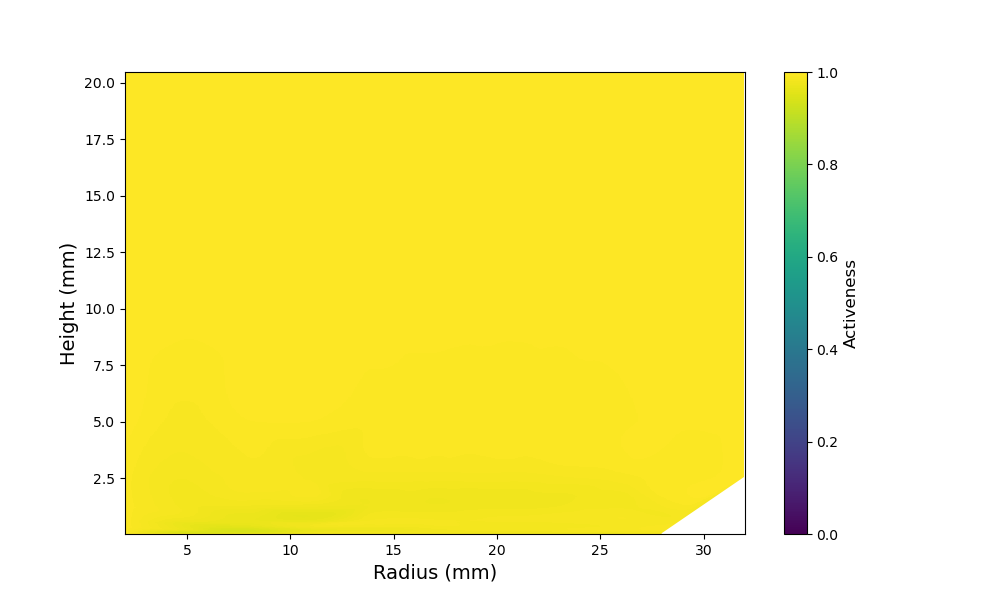
\includegraphics[trim={1.5cm 0cm 3.3cm 1cm},clip,width=0.49\linewidth]{ch5/figs/activeness_map_cubic_sc=0.0_ponama_1_5000_linear_full.png}
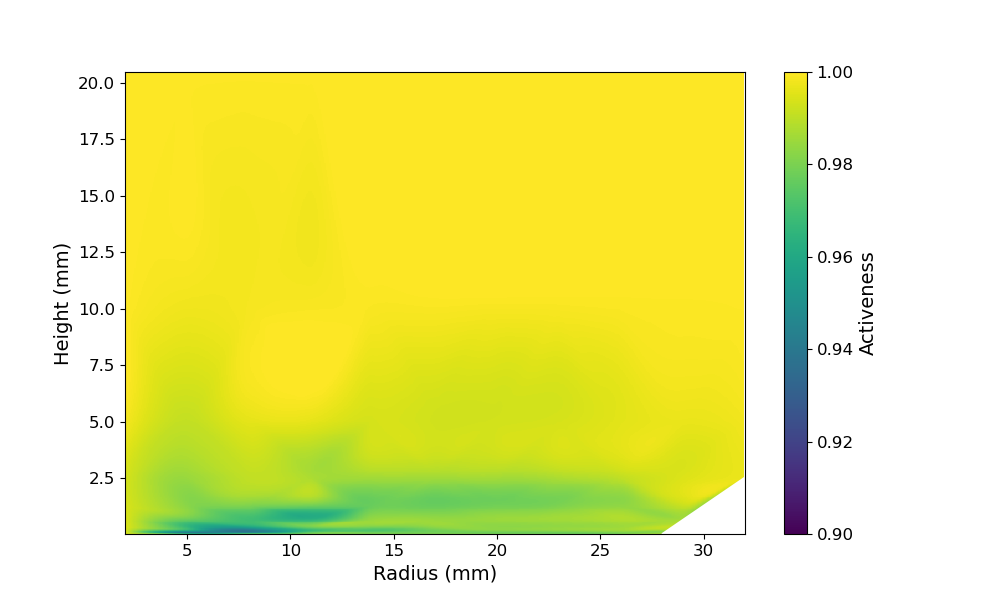
\includegraphics[trim={1.5cm 0cm 3.3cm 1cm},clip,width=0.49\linewidth]{ch5/figs/activeness_map_cubic_sc=0.0_ponama_1_5000_linear.png}
\caption{Interpolated activeness map for a PPC detector using \ehd with zero surface charge. Without surface charge there is nearly full collection. Right plot shows the same map with using narrow color scale.}
\label{ch5_fig_interpolated_activeness_map_0}
\end{figure}

Figure \ref{ch5_fig_interpolated_activeness_map_pos} shows the activeness map for positive surface charge. The loss of activeness is smaller than that for negative surface charges, since electrons are the minority charge carriers. Points at the same height but lower radii have a lower activeness because electrons must travel a longer distance, increasing the probability that they are pulled onto the surface by a negative surface charge.

\begin{figure}%[!htb]
\centering
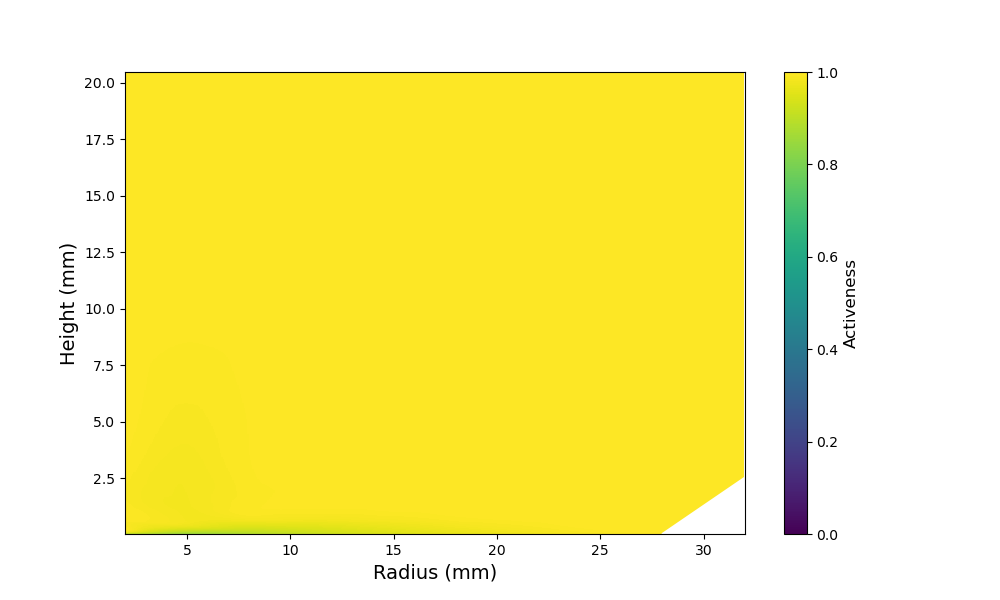
\includegraphics[trim={1.5cm 0cm 3.3cm 1cm},clip,width=0.49\linewidth]{ch5/figs/activeness_map_cubic_sc=0.3_ponama_1_5000_linear_full.png}
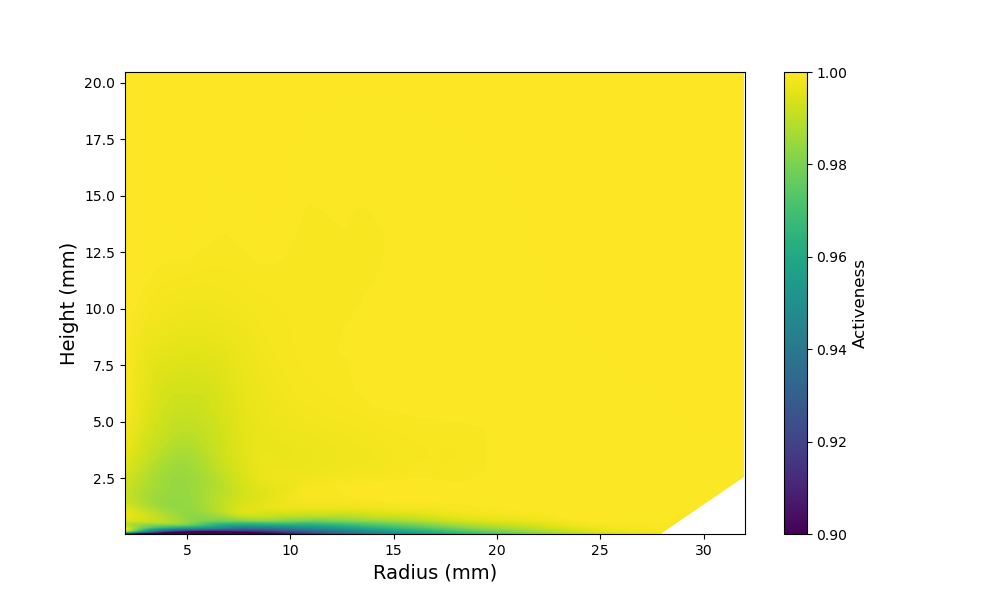
\includegraphics[trim={1.5cm 0cm 3.3cm 1cm},clip,width=0.49\linewidth]{ch5/figs/activeness_map_cubic_sc=0.3_ponama_1_5000_linear.png}
\caption{Interpolated activeness map for a PPC detector using \ehd with positive surface charge. The right plot is shown using narrow color scale. At a smaller radius, there is a higher chance of the electron component being pulled onto the surface causing higher loss of activeness. The activeness loss is smaller than negative surface charge since electrons are minority signal component.}
\label{ch5_fig_interpolated_activeness_map_pos}
\end{figure}

Figure \ref{ch5_fig_interpolated_icpc_activeness_map} shows the activeness maps for the Mirion ICPC detectors. The ICPC detectors have a smaller passivated surface and thus have a lower loss in activeness compared to the PPC detectors.  In addition, these detectors have a ditch feature at the passivated surface location, increasing the vertical component of the electric field in this region. This decreases the likelihood that charges are pushed to the surface of the detector in this remaining passivated surface region. Figure \ref{ch5_fig_elect_field_lines_surface_V07647A} shows the electric field near the detector ditch. The field lines suggest that this loss is primarily due to electrons being pulled in the ditch.

\begin{figure}%[!htb]
\centering
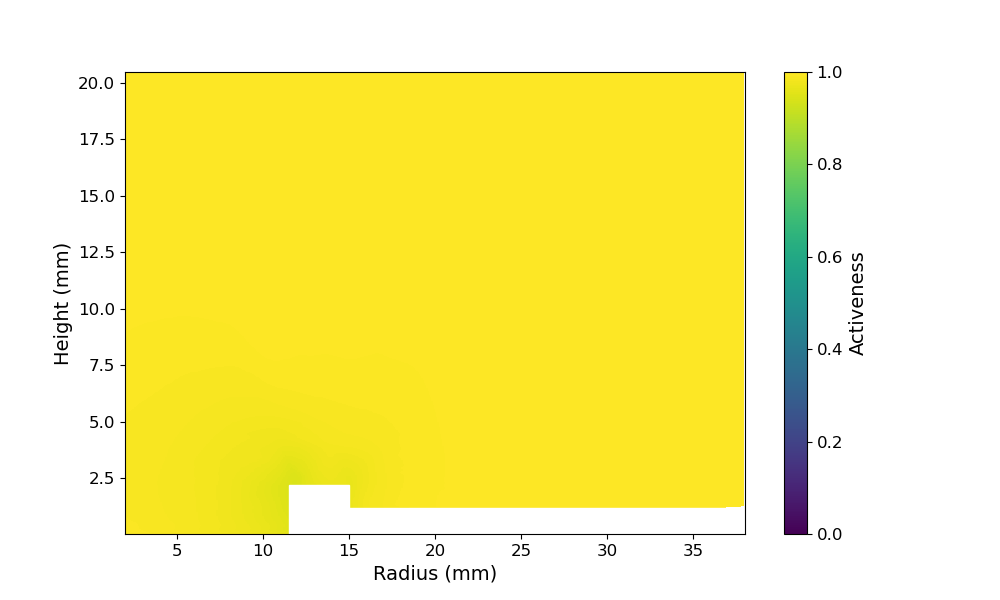
\includegraphics[trim={1.5cm 0cm 3.3cm 1cm},clip,width=0.49\linewidth]{ch5/figs/activeness_map_cubic_sc=-0.3_V07647A_5000_linear_full.png}
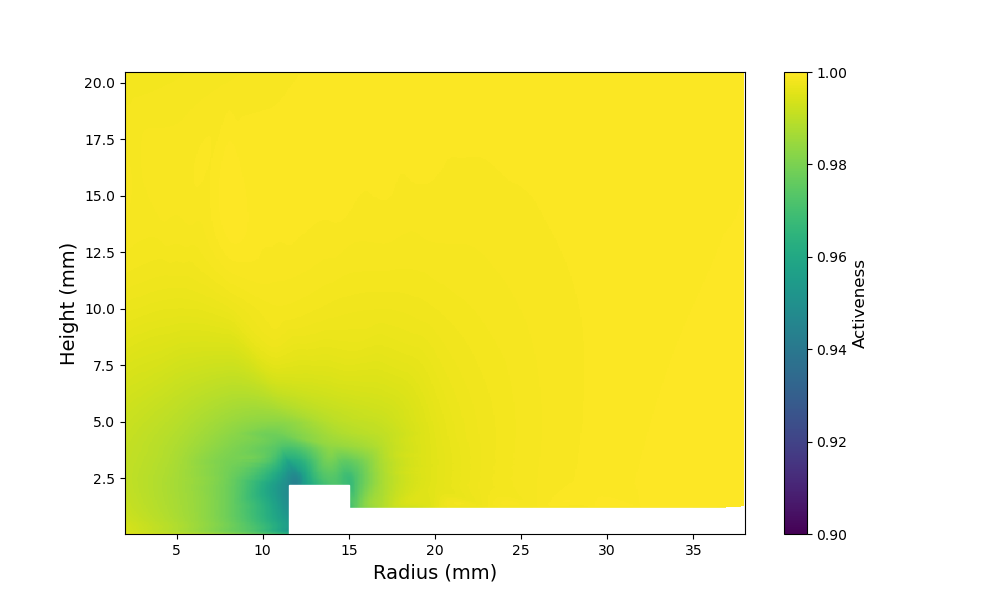
\includegraphics[trim={1.5cm 0cm 3.3cm 1cm},clip,width=0.49\linewidth]{ch5/figs/activeness_map_cubic_sc=-0.3_V07647A_5000_linear.png}

\caption{Interpolated activeness map for a Mirion ICPC detector using \ehd with negative charge. The right plot is show in a narrow color scale. The ICPC detector have significant less reduction in activeness than PPC detectors. The activeness loss also does not depend on the surface charge and the same activeness is found for positive and negative surface charge.}
\label{ch5_fig_interpolated_icpc_activeness_map}
\end{figure}


\section{\label{res:1} Reproduction of Results from Established Test Stands}
To validate EH-Drift against existing measurements, we modeled alpha events studied for a detector operated in the TUBE \cite{TUBE_paper} and GALATEA \cite{galatea_paper} scanning test stands. The {\ponama} detector (PPC from ORTEC made from Natural Material) is a research and development PPC detector manufactured by ORTEC using natural abundance Germanium. Its properties are given in table \ref{ch5_5_tab_ponama1_geometry}. The teams that took these measurements hypothesized that the difference in behavior observed between them was due to opposite-sign charge build-up on the detector's passivated surface. If this hypothesis is correct and the {\ehd} code is correctly modeling the charge collection behavior in this region, varying the surface charge in the model should allow for an accurate fit to both sets of data.

\begin{table}[htb]
\centering
\begin{tabular}{|l | l|}
\hline
Detector Geometry   & Value \\
\hline
Height      & 50.5\,mm  \\
Radius             & 34.5\,mm  \\
Point-contact height          & 2.1\,mm   \\
Point-contact radius         & 1.4\,mm   \\
Taper length               & 4.5\,mm   \\
Capacitance & 1.8\,pF \\
Depletion Voltage & 1850\,V \\
\hline
\end{tabular}
\caption{Key geometry dimensions for the {\ponama} detector.}
\label{ch5_5_tab_ponama1_geometry}
\end{table}



We simulated events using various surface charges in the {\ponama} detector.  We then fit those different curves to the data to estimate the surface charge needed to match the behavior observed in each measurement.

%We generated 8$\mu$s pulse using {\ehd} and applied a trap filter of 4$\mu$s rise time, 3$\mu$s flat-top time, and picked off energy at 7$\mu$s.
\begin{figure}%[!htb]
%[trim={left bottom right top},clip]
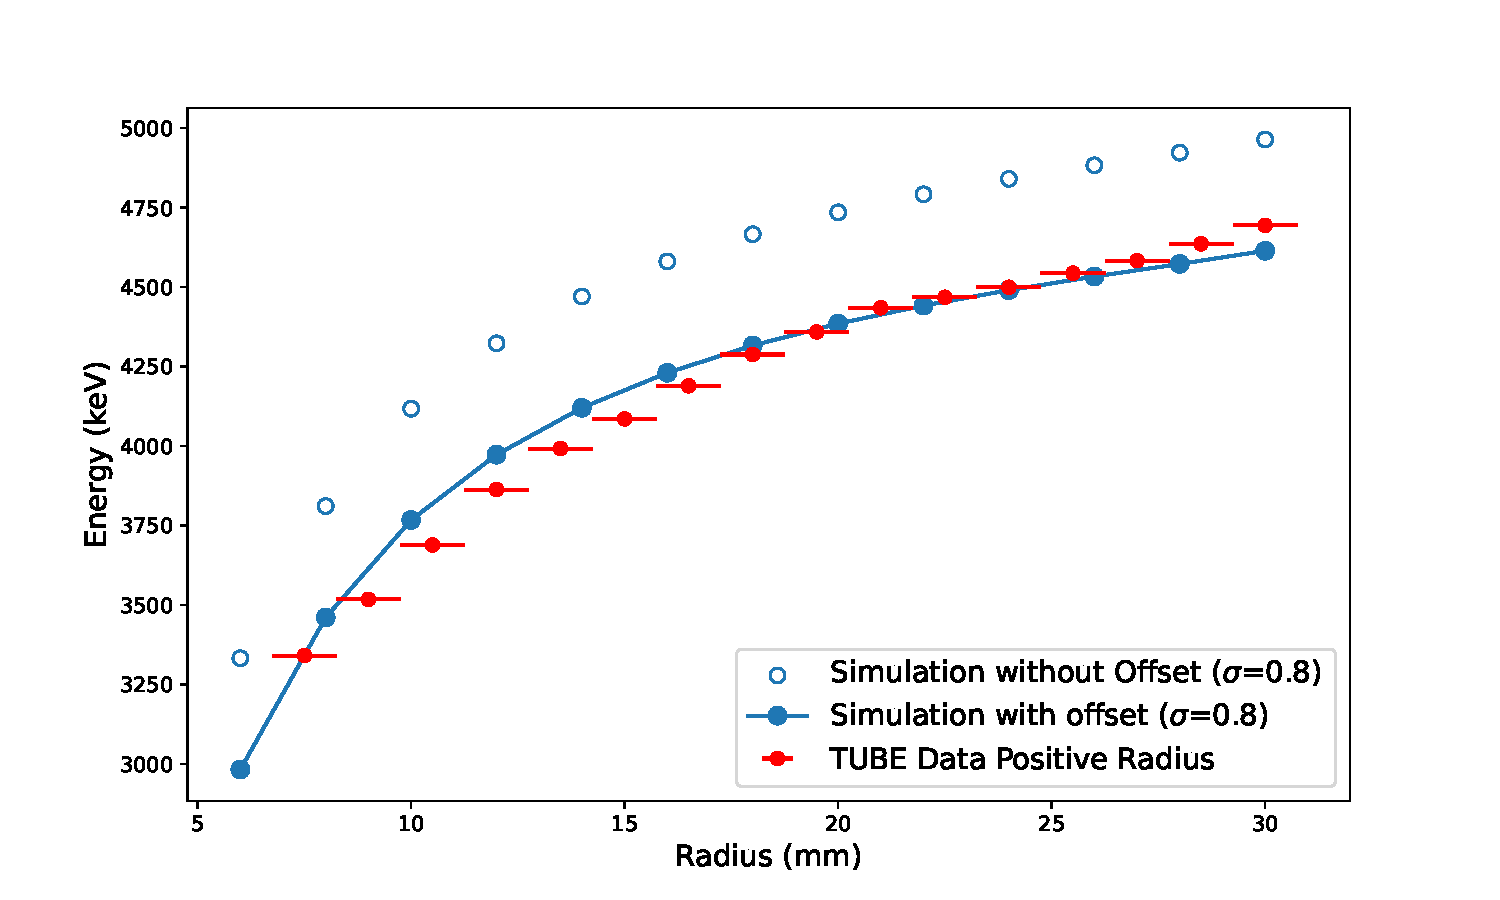
\includegraphics[trim={0.3cm 0.1cm 1.7cm 0.1cm},clip,width=\linewidth]{ch5/figs/tube_fit.pdf}
\caption{Fitting the activeness in the TUBE scanner with \ehd{}. A positive surface charge can help explain the increase in collected energy with radius. A $350$ keV energy offset and $2.0$ mm radial offset is needed to match the data, which could occur if there was a thin fully dead region either in the source or at the detector surface. Experimental values from \cite{TUBE_paper}}
\label{fig:tube_fit}
\end{figure}


\begin{figure}%[!htb]
\centering
%[trim={left bottom right top},clip]
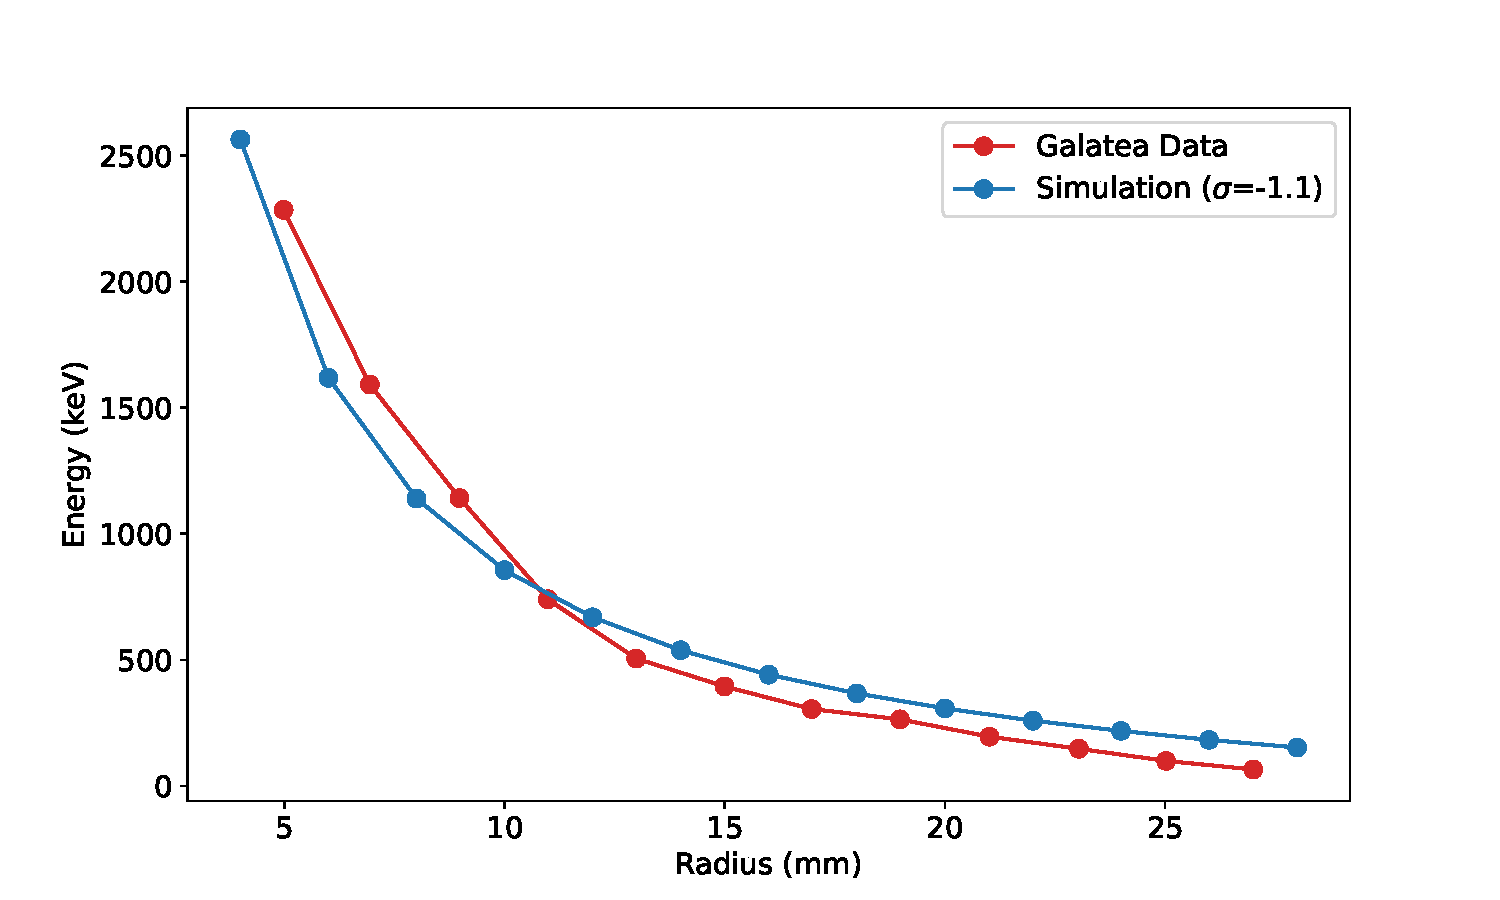
\includegraphics[trim={0.3cm 0.1cm 1.7cm 1cm},clip,width=\linewidth]{ch5/figs/gal_fit.pdf}
\caption{Fitting the activeness in GALATEA scanner with \ehd{}. A negative surface charge can help explain the decrease in collected energy with radius. Experimental values from \cite{galatea_paper}}
\label{fig:gal_fit}
\end{figure}

We found a positive surface charge that explains the behavior observed in TUBE. Figure \ref{fig:tube_fit} compares the TUBE scanner data with EH-Drift simulations with a positive surface charge. A positive surface charge would attract electrons on the surface, resulting in energy degradation. In this scenario, electrons are collected at the n+ surface, so the closer the points are to the origin, the more chance there is for the electrons to get trapped onto the surface and the more energy degradation there is. Thus, the energy collected is proportional to the radius. Although the simulations have matched the trend well, an offset of $350$ keV in energy and $2.0$ mm in radius offset is required to match the data. This could be because the source beam used in TUBE had an uncertainty of about $0.75$ mm in radial position. There could also be a thin dead layer either within the source used or at the detector surface, before the passivated surface. We added an energy offset to account for this offset.

In the GALATEA scanner, the significantly different behavior can be explained using a negative surface charge as shown in figure \ref{fig:gal_fit}. The negative surface attracts holes to the surface, and since the holes are collected at the point contact, located at r=0, the higher the radius, the more charges end up on the surface. Thus, the collected energy falls inversely with the radius.

\section{Efficiency Estimations in the Region of Interest}
\label{ch5_res_efficiency} 
We can use the maps created by {\ehd} to estimate the efficiency of {\onbb} event collection. LEGEND's search for {\onbb} is conducted by fitting a peak to events at Q$_{\beta \beta}$, the shape of which is determined from the energy resolution of the detector. Only events falling in this narrow peak would be counted as {\onbb} signal events. However, if an event occurs close to the passivated surface, there is a chance that the collected energy would be degraded enough to not register as an event in the Region of Interest (ROI). Standard calculations of the detector's active volume that account for the loss of efficiency from regions of partial charge collection do not include any passivated surface effects. 

To understand this effect, we created activeness maps for detectors with a $2039$ keV initial energy, which is the Q value of {\onbb} in Germanium. We did this for various surface charges. We then randomly sampled $20,000$ points uniformly in the detector and estimated their activeness using the interpolated map. A threshold of $3$ keV is defined for the ROI, which means that if the activeness at a point reduces the measured energy of the simulated {\onbb} event below 2036 keV, that event is not registered as a {\onbb} event. For this initial study, this threshold $3$ keV is chosen as an approximation for the peak width used to fit {\onbb} events, since the average FWHM of the detectors in LEGEND is roughly $2.5$ keV.  Each point is assigned a value of $1$ if an event at that location is counted as {\onbb}, or $0$ otherwise. Figure \ref{ch5_fig_binary_activenss} shows this binary activeness for a PPC and Mirion ICPC detector with negative surface charge. The overall efficiency is then calculated as the sum of activeness values divided by the total number of points, while factoring in the azimuthal angle dependence.

\begin{table}[!htb]
    \centering
    \begin{tabular}{|l|c|c|c|}
    \hline
    Surface Charge & V07647A & {\ponama} & P00698A \\
    ($\times$ {\scunit}) & (\%) & (\%) & (\%) \\
    \hline
    $-0.30$ & 99.82 & 83.80 & 95.21 \\
    $-0.15$ & 99.82 & 87.78 & 97.25 \\
    $-0.03$ & 99.82 & 95.34 & 98.85 \\
    $\phantom{-}0.00$ & 99.82 & 99.02 & 99.91 \\
    $\phantom{-}0.03$ & 99.82 & 99.98 & 99.98 \\
    $\phantom{-}0.15$ & 99.82 & 99.88 & 99.90 \\
    $\phantom{-}0.30$ & 99.82 & 99.76 & 99.71 \\
    \hline
    \end{tabular}
        \caption{Estimated {\onbb} efficiency for three different germanium detectors at different surface charges.}
        \label{ch5_tab_efficiency_surface_charge}
    
\end{table}


\begin{figure}%[!htb]
\centering
%[trim={left bottom right top},clip]
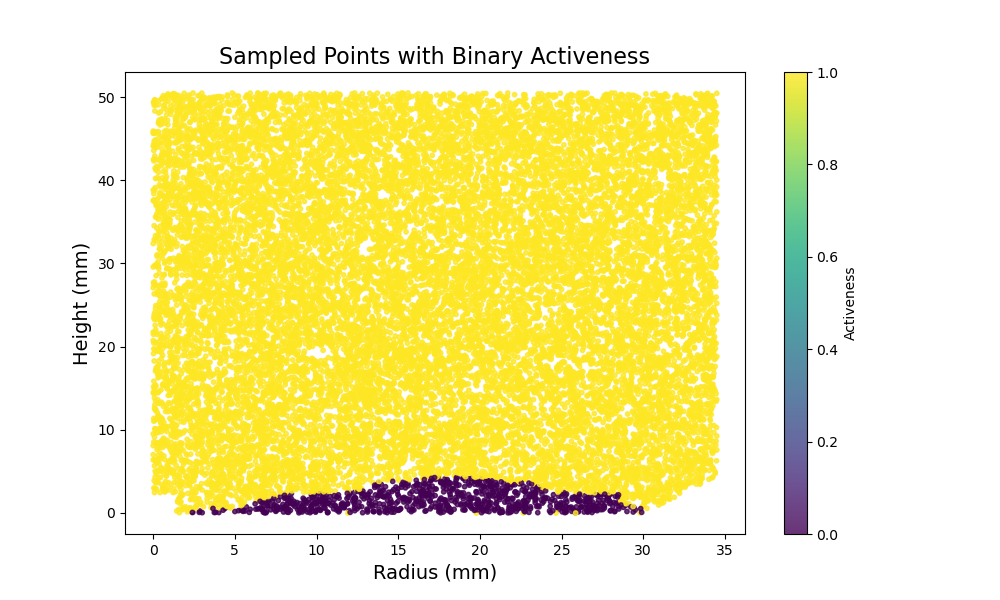
\includegraphics[trim={1.5cm 0cm 6cm 1.77cm},clip,width=0.49\linewidth]{ch5/figs/bianry_act_ponama_1_-0.03.png}
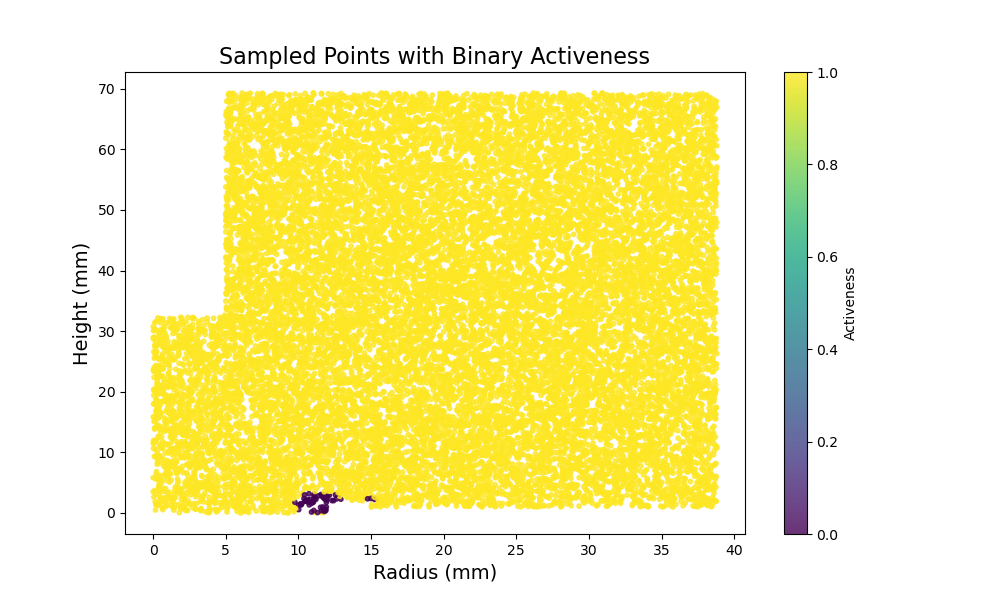
\includegraphics[trim={1.5cm 0cm 6cm 1.77cm},clip,width=0.49\linewidth]{ch5/figs/bianry_act_V07647A_-0.03.png}
\caption{Binary activeness for {\ponama} detector and Mirion ICPC detector with negative surface charge. A $3$ keV energy resolution threshold is defined. If energy is degraded above it, it is labeled zero, else 1. The purple dots show where {\onbb} events would be not be recorded for the detectors.}
\label{ch5_fig_binary_activenss}
\end{figure}

Table \ref{ch5_tab_efficiency_surface_charge} summarizes the results of the study for the {\ponama} detector, a LEGEND PPC detector, and a Mirion ICPC detector. Figure \ref{fig:efficiency_sc_plot} plots the efficiency against the surface charge. The efficiency drops rapidly for negative surface charges in both PPC detectors; however, it decreases most sharply for {\ponama}, which has a lower depletion voltage and thus a weaker electric field near the surface. The LEGEND PPC detector also loses efficiency quickly due to its larger passivated surface, but its higher electric field moderates the overall loss more than in {\ponama}.

\begin{figure}%[!htb]
\centering
%[trim={left bottom right top},clip]
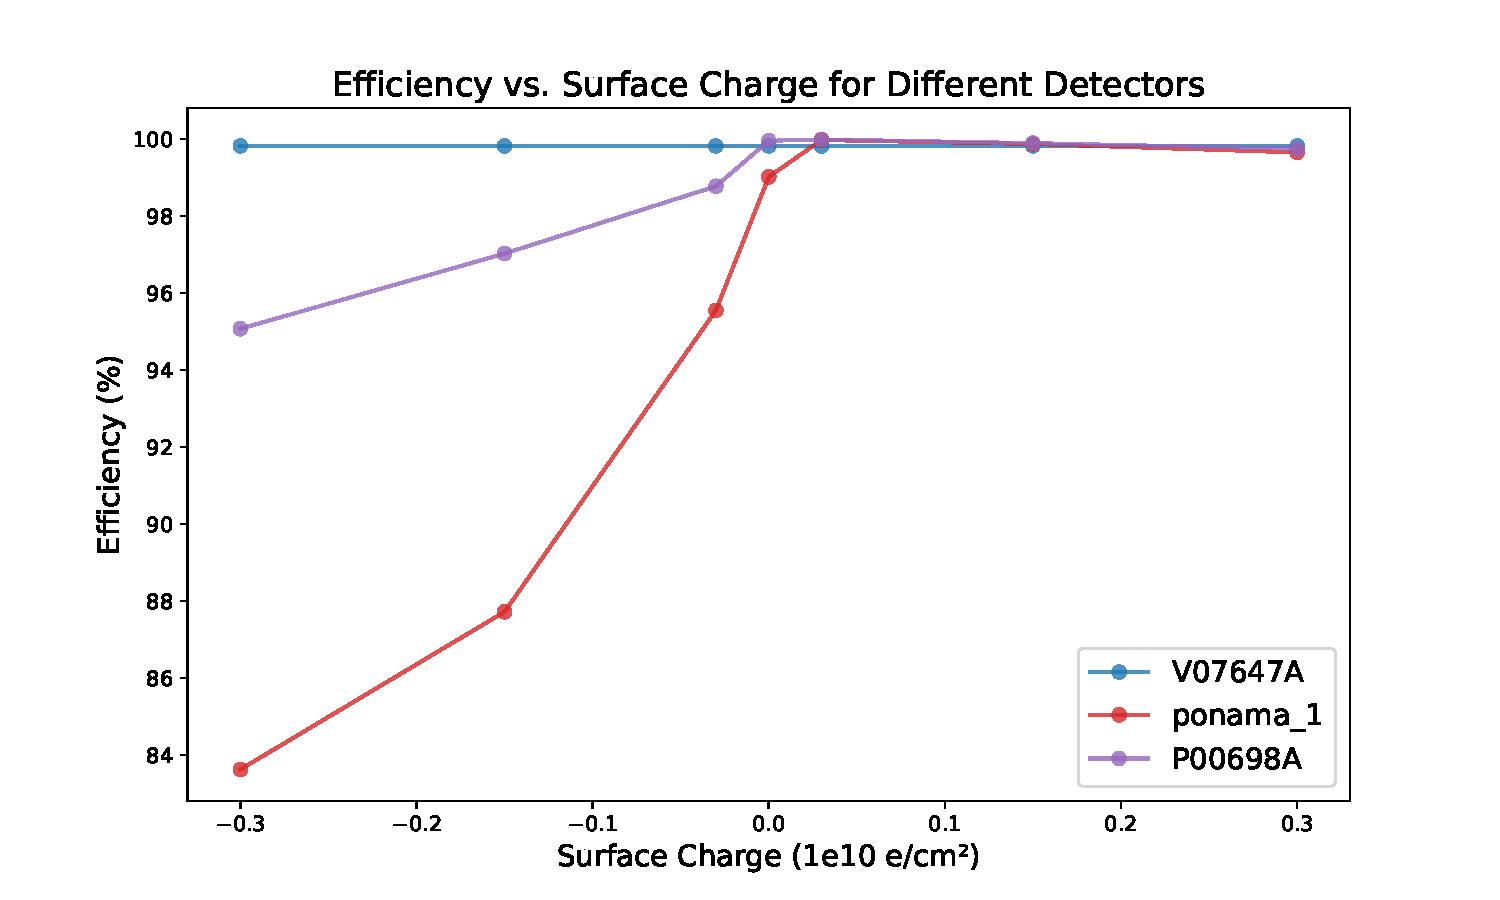
\includegraphics[trim={1.6cm 0.3cm 2cm 1.8cm},clip,width=\linewidth]{ch5/figs/efficiency_0nbb.pdf}
\caption{Efficiency in the ROI versus surface charge calculated using the binary activeness.}
\label{fig:efficiency_sc_plot}
\end{figure}

The Mirion-style ICPC detector exhibits virtually no reduction in activeness, primarily because it has a much smaller passivated surface. The collection efficiency is $99.82\%$. To understand this slight reduction in efficiency, one can look at the electric field in the ditch of the detector shown in figure \ref{ch5_fig_elect_field_lines_surface_V07647A}. The field lines indicate that the electron component, which drifts opposite to the field lines, near the surface will be pulled onto the ditch, which is passivated. This loss in activeness is much smaller than in other types of detectors. Since LEGEND-1000 plans to use only Mirion-style ICPC detectors, surface backgrounds in that experiment are expected to be significantly reduced.

\begin{figure}%[!htb]
\centering
%[trim={left bottom right top},clip]
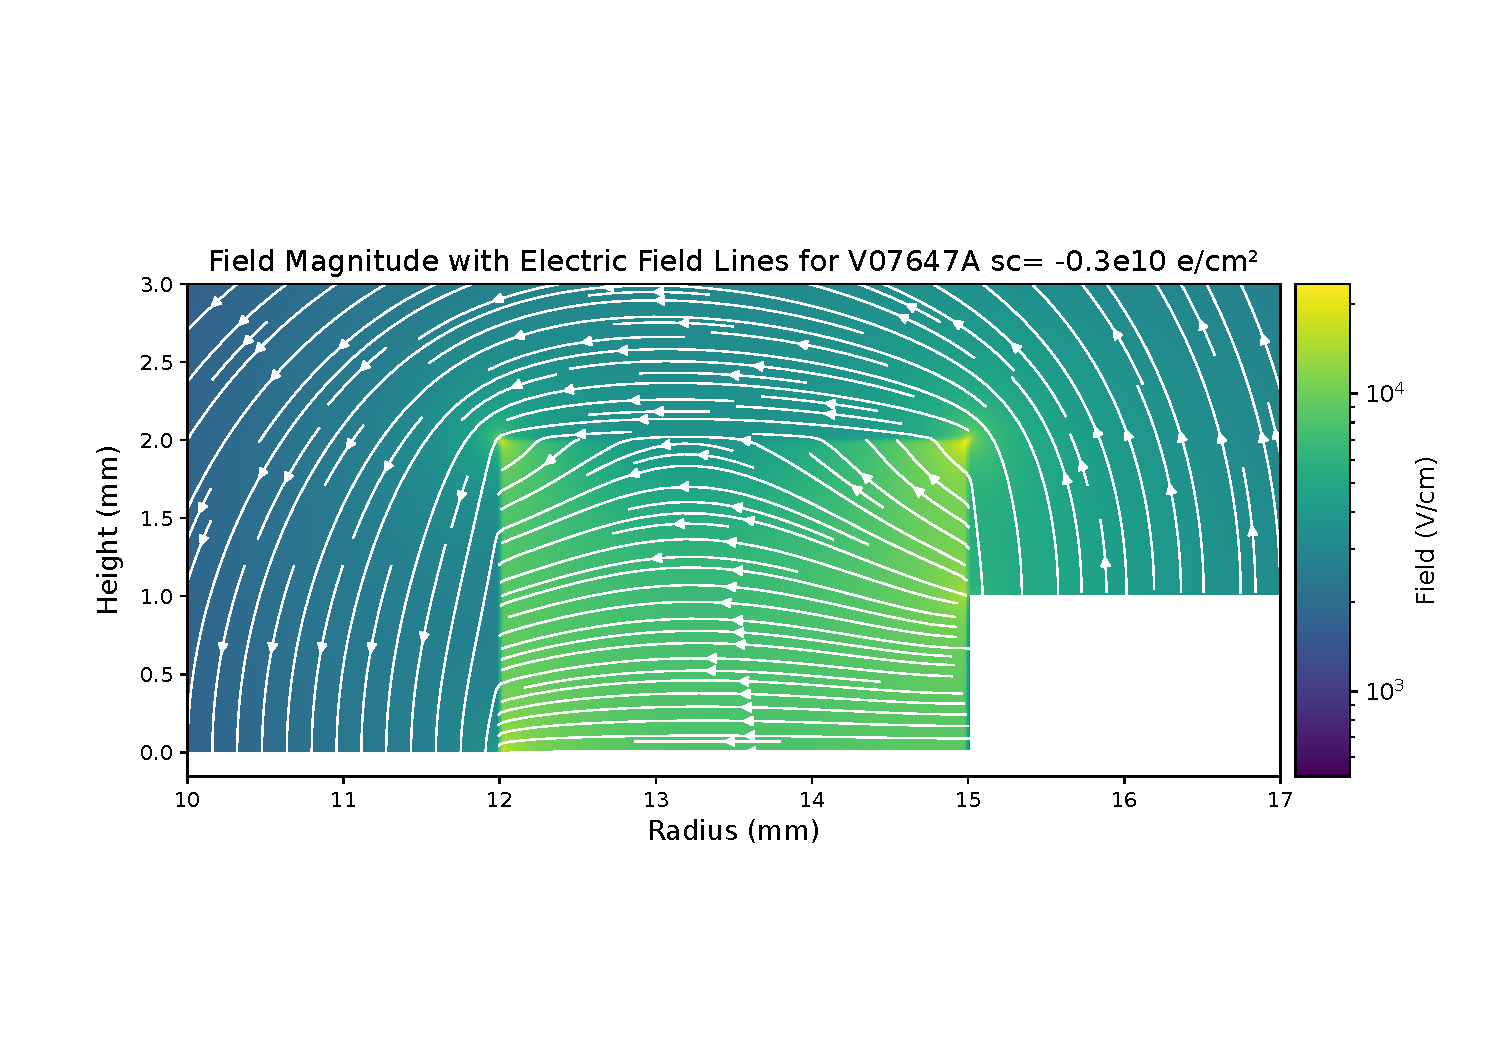
\includegraphics[trim={0cm 3cm 0cm 4.69cm},clip,width=0.99\linewidth]{ch5/figs/elect_field_lines_surface_V07647A_sc_-0.3.pdf}
\caption{Electric magnitude and field lines near the ditch of a Mirion ICPC detector with negative surface charge. In Mirion ICPC, the flat p$^+$ point contact, where the field lines end, extend to the start of ditch at r=$12$. The n$^+$ contact starts at end of ditch at r=15, shown by the origin of field lines. The field lines attract electron component to the surface which drift slowly. The reduction in activeness is fraction of other detector geometries.}
\label{ch5_fig_elect_field_lines_surface_V07647A}
\end{figure}


\section{\label{res:3} Generating Background Spectra}
Geant4 is a Monte Carlo-based toolkit that can simulate the passage of particles through matter. To demonstrate how EH-Drift can be used to create spectral components for background modeling, we performed a {\geant} simulation of the {\ponama} detector exposed to a planar $5$ MeV alpha source. We recorded the resulting hits from alpha particles entering the detector. We then used the activeness map to estimate the energy that would be collected from surface effects. Figure \ref{fig:eng_spec_degradation} shows what the collected energy spectrum would look like for various surface charge scenarios. In particular, the spectrum for the negative surface charge closely matches the alpha spectra observed in the {\MJD} experimental data and initial background modeling for PPC detectors in the LEGEND data.

\begin{figure}%[!htb]
  \centering
      %[trim={left bottom right top},clip]
  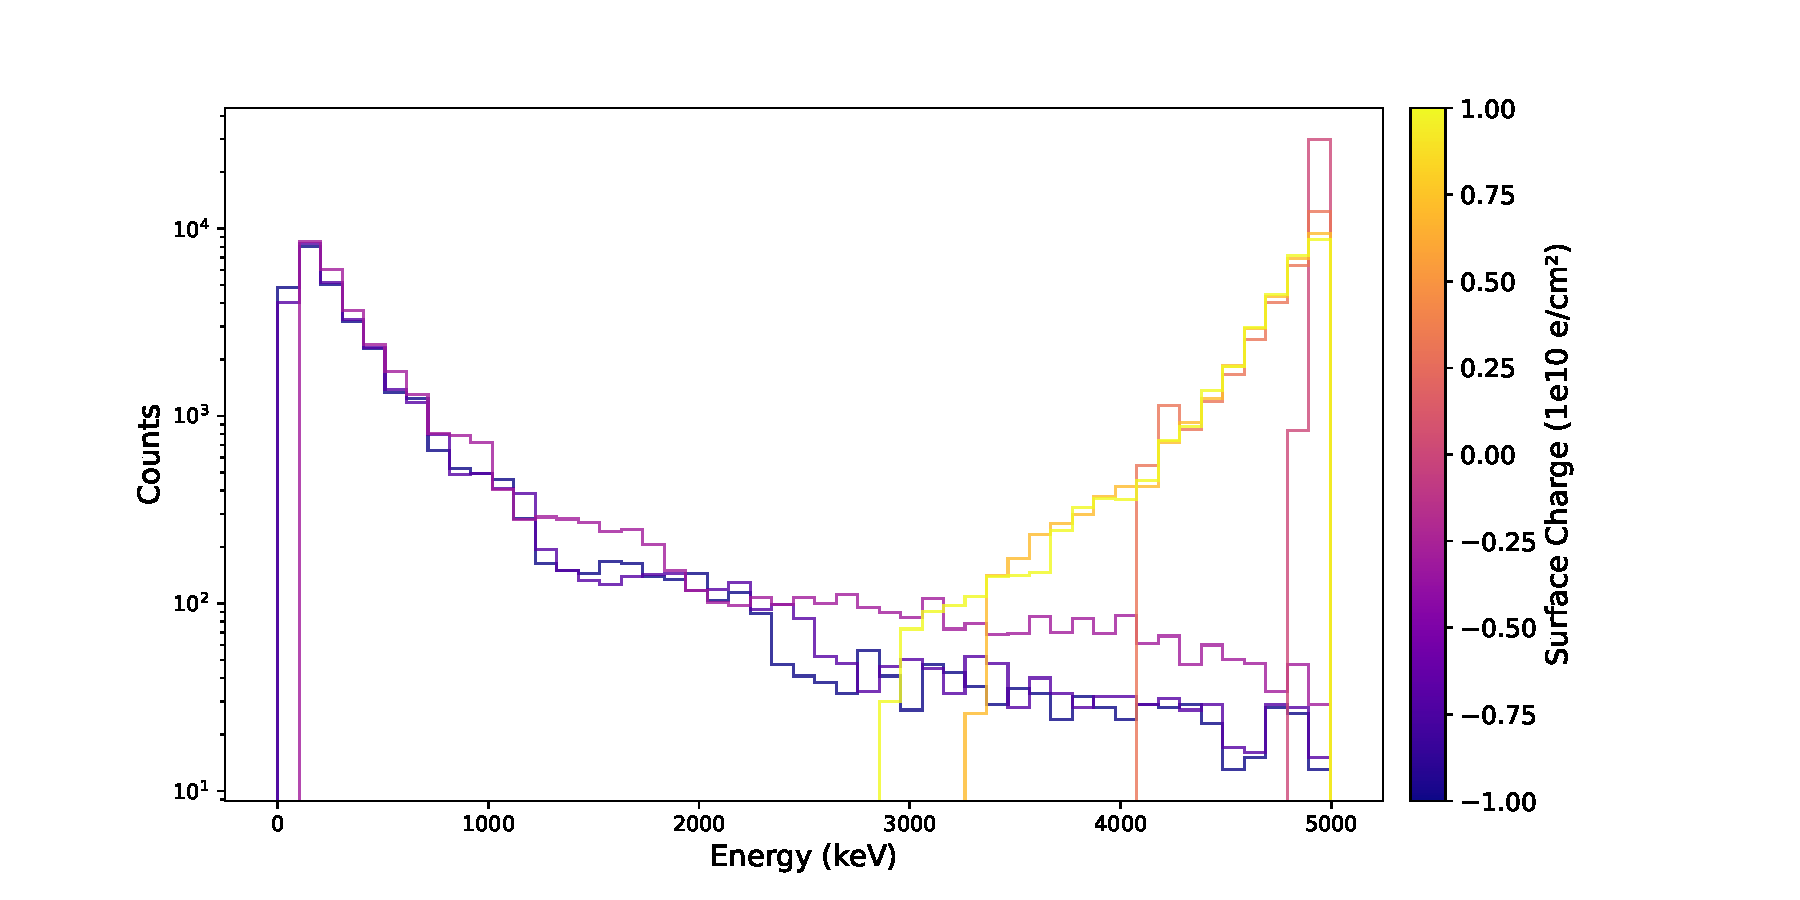
\includegraphics[trim={2cm 0.5cm 3.5cm 1.7cm},clip,width=0.99\linewidth]{ch5/figs/eng_deg_hist.pdf}
  \caption{Degradation of the alpha-particle energy spectrum under various surface charges. The location of hits of alpha particles were generated using a {\geant} simulation of planar alpha source of 5\,MeV on {\ponama} detector. Energy degradation for an alpha event was calculated from interpolated map for each surface charge. The unit of surface charge is in {\scunit}.}
  \label{fig:eng_spec_degradation}
\end{figure}

To understand the effect of the passivated surface on beta decays such as those that form a significant background in LEGEND, we simulated the spectrum of $^{42}$K using {\geant} for {\ponama} detector. The output energy spectrum is shown by the blue histogram in figure \ref{ch5_figs_k_42_degrad}. The spectrum has a prominent gamma line at 1500 keV and a broad beta continuum extending to 3500 keV, which is the Q-value of the decay. Using {\ehd} we estimate the activeness of the passivated surface assuming a $2039$ keV energy map and a surface charge of $- 0.5 \times$ {\scunit}. The resulting spectrum is shown by the yellow curve.

\begin{figure}%[!htb]
  \centering
      %[trim={left bottom right top},clip]
  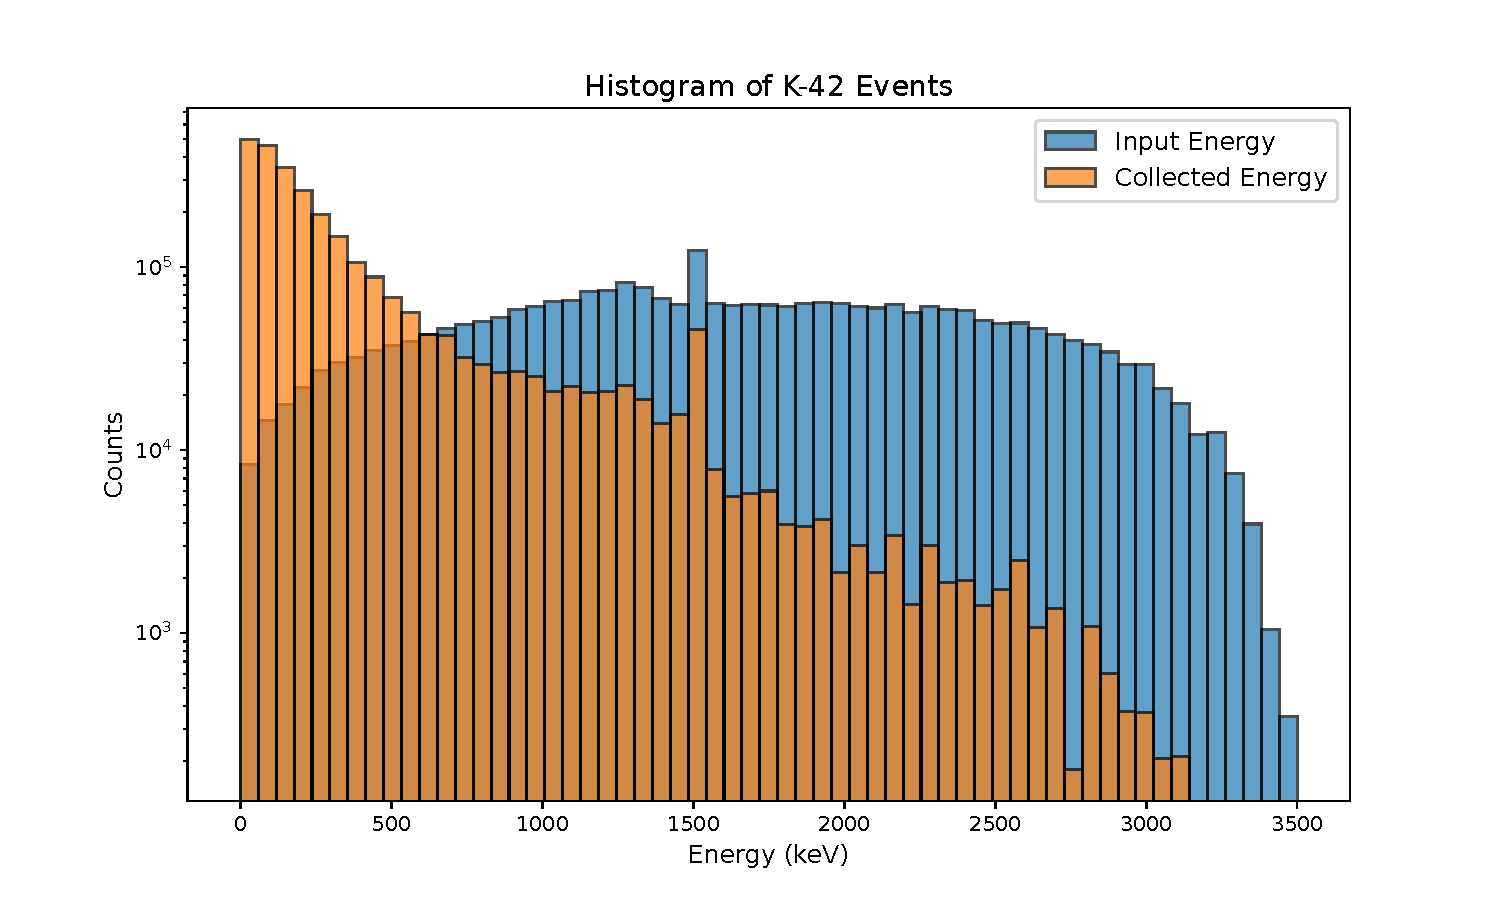
\includegraphics[trim={1.5cm 0.0cm 2cm 1.76cm},clip,width=0.99\linewidth]{ch5/figs/k_42_beta_spectrum.pdf}
  \caption{Degradation of the K-42 energy spectrum in {\ponama} detector. The detector surface had a surface charge of $- 0.5 \times$ {\scunit}. The activeness was calculated assuming $2039$ keV energy map. This result does not include a model for the dead layer created by the lithiated n$^+$ contact.}
  \label{ch5_figs_k_42_degrad}
\end{figure}

These two preliminary results, along with the dramatic active-volume effects for {\onbb} signal efficiency, show the importance of incorporating the results of the {\ehd} simulations into the LEGEND background model.